

\section{Evaluation}

\begin{figure*}[htb]
  \centering
  \begin{tabular}{c}
  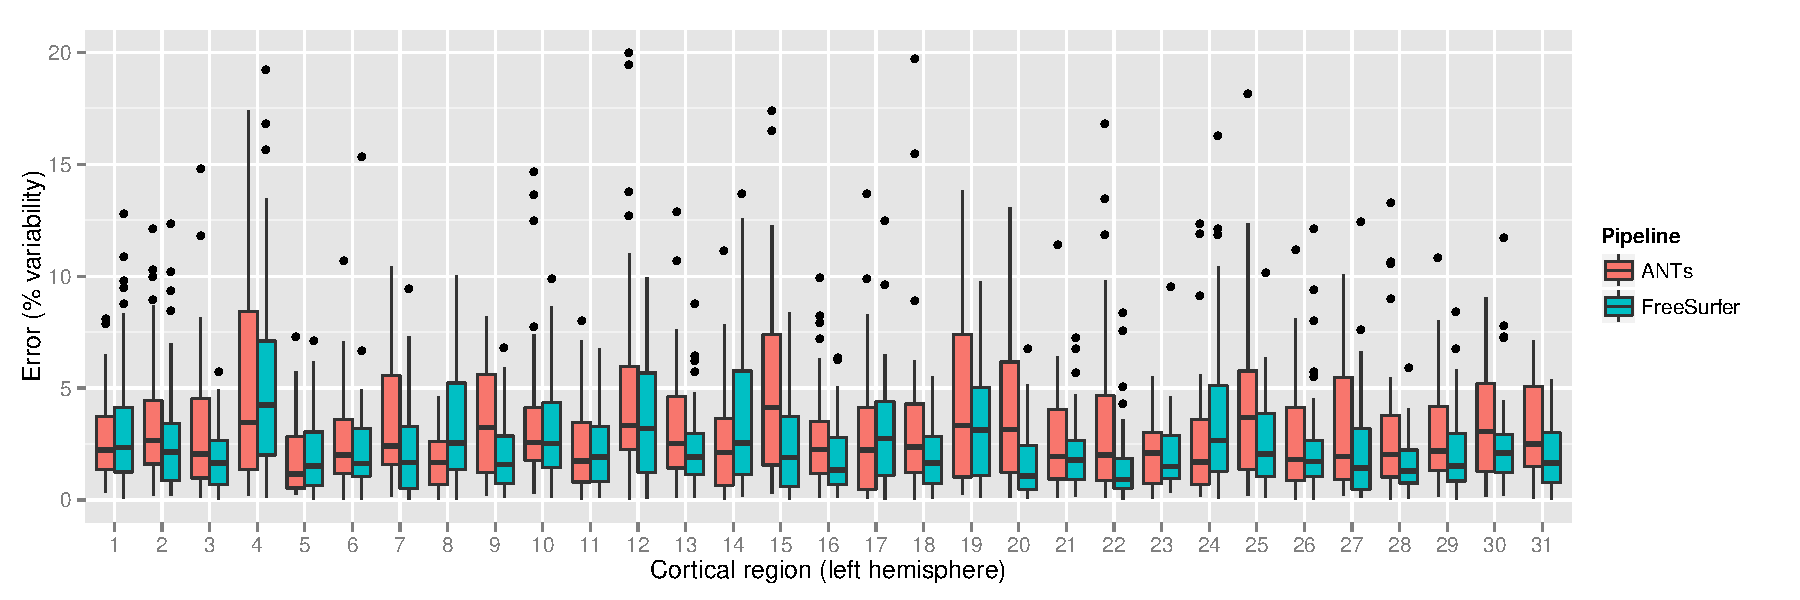
\includegraphics[width=160mm]{repeatabilityLeft.pdf} \\
  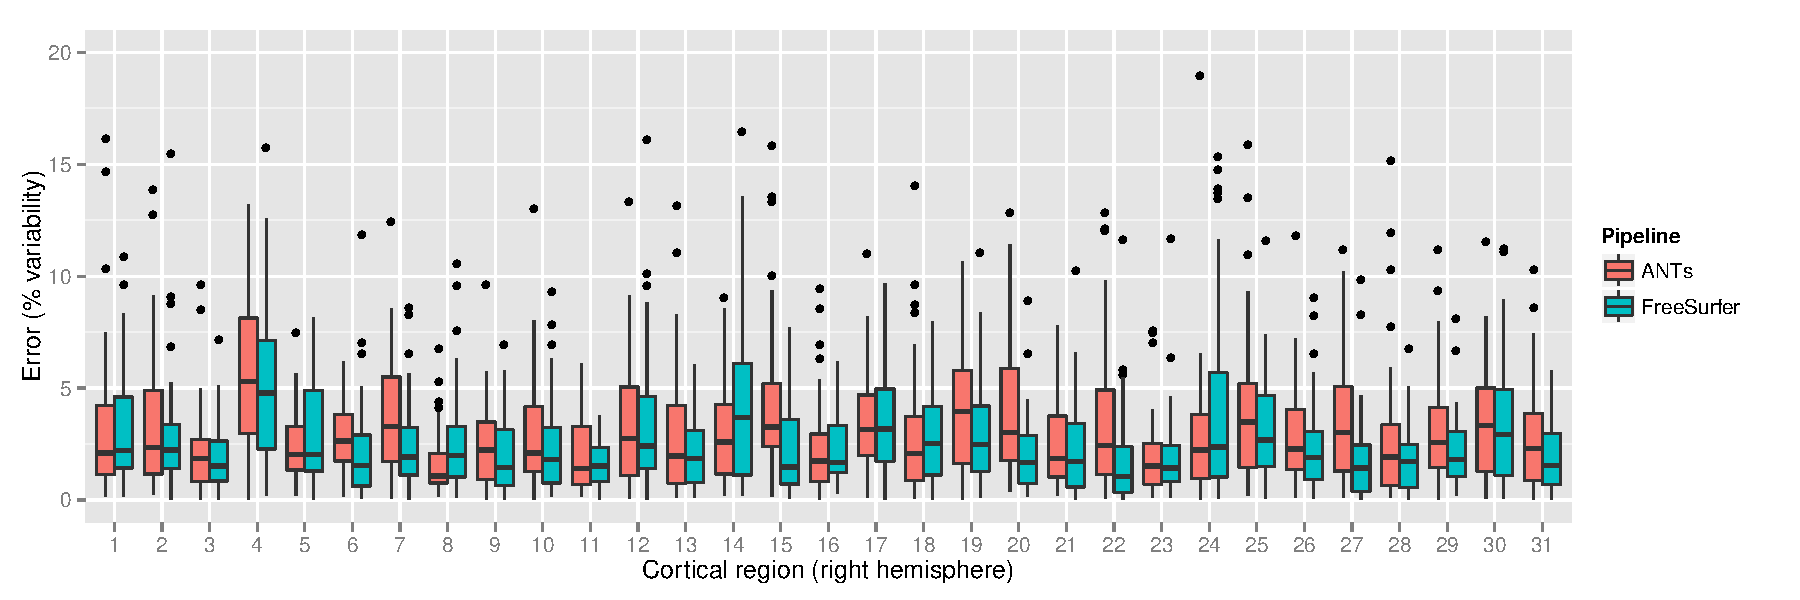
\includegraphics[width=160mm]{repeatabilityRight.pdf}
  \end{tabular}
  \caption{Percent error variability for both ANTs and FreeSurfer pipelines 
           over the left and right hemispheres of both the MMRR and OASIS
           data subsets within the 62 regions defined by the
           Desikan-Killiany-Tourville atlas.  Both methods demonstrate good repeatability
           qualities.
           }
  \label{fig:repeatability}
\end{figure*}


Traditional assessment approaches, such as manual
labeling, are inadequate for evaluating large-scale performance.  
We therefore sought to minimize failure rate, quantify the repeatability of cortical
thickness measures, and
determine whether the ANTs pipeline reveals biologically plausible relationships
between the cortex, gender,%
\footnote{
We recognize the distinction often made between ``sex'' and ``gender'' 
(cf {\tt http://www.who.int/gender/whatisgender/en/}).
As the demographic information collected during the course of the imaging studies 
is presumably self-reported, we assume that most self-identify in terms of 
gender and, therefore, use the term ``gender'' in data
descriptions.
}
and age and how its performance compares
to the current de facto standard of FreeSurfer-derived thickness estimation.
Collectively, these surrogate
measurements allow us to establish data-derived relative performance standards.
Additionally, for completeness, we include timing results as that factors into
usability.

\subsection{Repeatability}%


Repeat scans of 40 subjects (20 MMRR subjects and 20 OASIS subjects) were 
used to determine the repeatability of regional cortical thickness 
measurements, $T$.  Similar to the reproducibility 
assessment given in \cite{jovicich2013}, we
demonstrate this in terms of the percent variability error:
\begin{align}
\varepsilon = \frac{|T_{scan} - T_{rescan}|}{0.5 \times (T_{scan} + T_{rescan})}.
\end{align}
Comparison of the ANTs and FreeSurfer percent variability errors for the 62 DKT 
regions for both the OASIS and MMRR scan-rescan data sets
are given in Figure \ref{fig:repeatability}.  Mean values are given in Table \ref{table:error}.
Although the variance is slightly greater 
for the set of ANTs measurements, statistical testing per cortical region 
(two-tailed paired t-test, corrected using false discovery rate) did not indicate 
non-zero mean differences for either approach for any region.


\begin{table}
\caption{{\color{blue}Mean repeatability error over all regions.}}
\label{table:error}
\centering
\begin{tabular*}{0.475\textwidth}{@{\extracolsep{\fill}} l c c}
\toprule
{} &        {\bf MMRR}  &  {\bf OASIS} \\
\midrule
{\color{blue}ANTs} &       3.2\%   &      3.3\% \\
{\color{blue}FreeSurfer} & 2.5\%   &       2.8\% \\
\bottomrule
\end{tabular*}
\end{table}

We also calculated the intraclass correlation coefficient 
(``ICC(2,1)'' in the notation of \cite{shrout1979}) to assess 
scan/rescan reliability. The ANTs thickness pipeline produced an 
ICC value of 0.98 and the FreeSurfer thickness pipeline yielded
an ICC value of 0.97, indicating good scan/rescan reliability for
both ANTs and FreeSurfer.

\subsection{Age prediction assessment}

Despite good repeatability with both ANTs and FreeSurfer, such measures
do not provide an assessment of accuracy or even relative utility.  For example, 
strong priors can yield good repeatability measures but potentially at the expense 
of data fidelity thus compromising the quality of models (statistical or otherwise) 
built from such results.  Given that ground truth is not available for 
these data nor for the many studies looking at brain
morphology, an indirect method (or set of methods) is required for
determining the quality of thickness estimation.

\begin{figure*}[htb]
  \centering
  \begin{tabular}{c}
  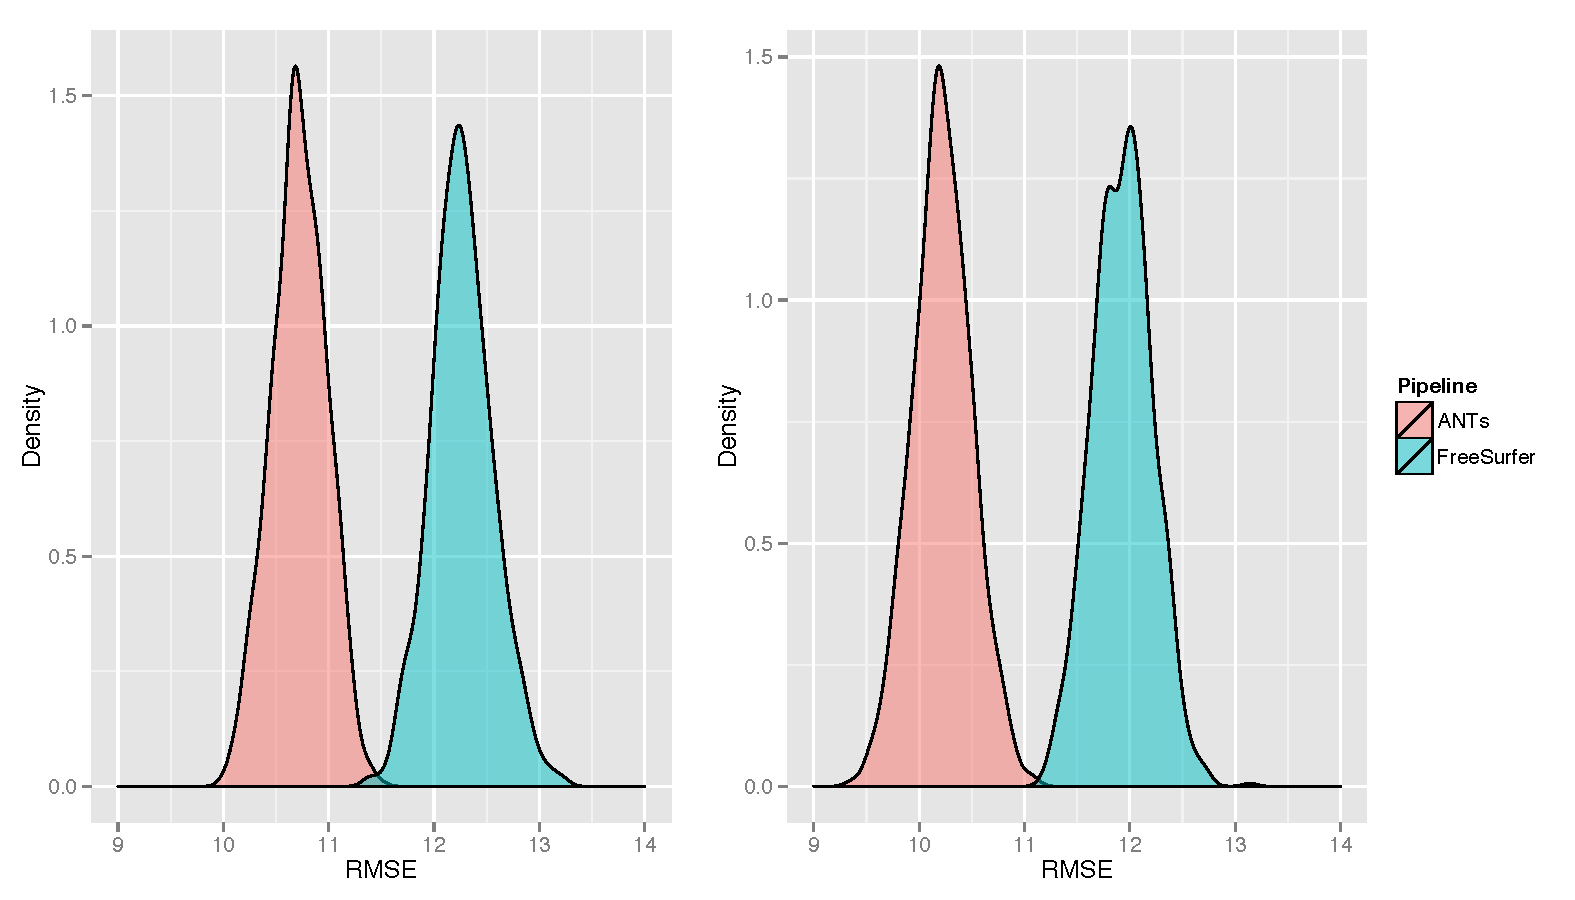
\includegraphics[width=140mm]{agePrediction.pdf} 
  \end{tabular}
  \caption{Age prediction RMSE distributions of linear (left) and random forest (right)
           models for the ANTs- and FreeSurfer-derived thickness values over the combined four             
           cohorts.  For both prediction
           models ANTs RMSE error is lower.
           }
  \label{fig:agePrediction}
\end{figure*}


For our first assessment, we modeled age versus regional cortical thickness values 
to determine which framework produces better predictive thickness estimates.  We first
subdivided the thickness data into training and testing subsets with an even split
between the two subsets.%
\footnote{
We tried various training proportions between 10 and 90\% (in increments of 10\%)
to see if that had an effect on relative performance for both age and 
gender prediction comparisons. Although age predictive capabilities for 
both pipelines showed improvement (gender prediction was mostly unaffected), 
the relative outcomes were the same.  
}
We then used the training data to create two models for each pipeline:
1) standard linear regression
and 2) random forests (a non-parametric machine learning technique) \citep{breiman2001},
for estimating age from both ANTs and FreeSurfer thickness values in the testing data.  

\begin{table}[htb]
\caption{Mean RMSE for age prediction in years.}
\label{table:agePrediction}
\centering
\begin{tabular*}{0.475\textwidth}{@{\extracolsep{\fill}} l c c}
\toprule
{} &        {\bf Linear Model}  &  {\bf Random Forest} \\
\midrule
ANTs (Combined) &       10.7   &       10.2 \\
FreeSurfer (Combined) & 12.3   &       11.9 \\
\midrule
ANTs (IXI) &       9.3   &       8.6 \\
FreeSurfer (IXI) & 12.3   &       11.7 \\
\midrule
ANTs (NKI) &       NA$^\dagger$   &       10.9 \\
FreeSurfer (NKI) & NA$^\dagger$   &       13.3 \\
\midrule
ANTs (OASIS) &       15.0   &     12.4 \\
FreeSurfer (OASIS) & 15.0   &       11.4 \\
\bottomrule
{\scriptsize $^\dagger$Fitting error.}
\end{tabular*}
\end{table}


The formula (in the notation of \cite{wilkinson1973}) for the linear model is
\begin{align}
  \label{eq:lmage}
  AGE \sim VOLUME + GENDER + \sum_{i=1}^{62} T(DKT_{i})
\end{align}
where $T(DKT_{i})$ is the average thickness value in region $DKT_{i}$ {\color{blue}{
and $VOLUME$ is total intracranial volume}}.
Similarly, the random forest 
model was specified as a combination of all terms
using the {\tt randomForest}%
%\footnote{
%http://cran.r-project.org/package=randomForest
%}
package in R with the default settings and 200 trees.

In order to ensure a fair comparison, the procedure described above consisting
of training and testing steps was performed for $n = 1000$ permutations to elicit a 
performance distribution which we measure using the relative mean square
error (RMSE):
\begin{align}
  RMSE = \sqrt{\frac{\sum \left(AGE_{true} - AGE_{predicted} \right)^2}{N}}.
\end{align}
{\color{blue}{Due to the limited range in ages across data sets, we restricted training
and testing to the age range $[20,80]$.  The resulting distributions are 
illustrated in Figure \ref{fig:agePrediction}.  In addition to a combined
assessment, we also perform separate model prediction for each of the three 
larger data sets (i.e., IXI, NKI, and OASIS).}}

%\begin{figure}[!h]
%  \centering
%  \begin{tabular}{c}
%  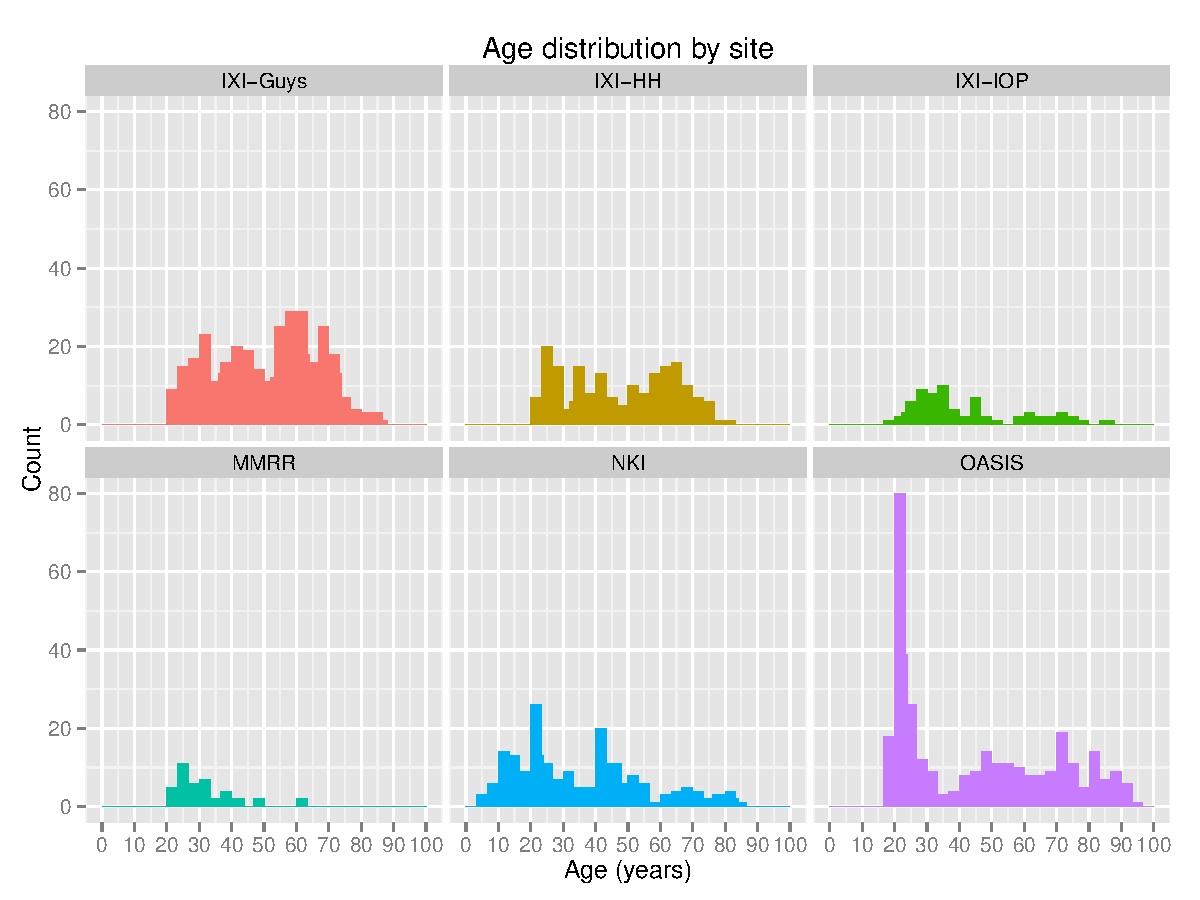
\includegraphics[width=87.5mm]{ageDistribution.pdf} 
%  \end{tabular}
%  \caption{Age 
%           }
%  \label{fig:ageDistribution}
%\end{figure}

ANTs-based RMSE values were lower for both models and each of the four
different subset comparisons except for the random forest model constructed
from the OASIS data set. 
All mean RMSE values are provided in Table \ref{table:agePrediction}.

\begin{figure}
  \centering
  \begin{tabular}{cc}
  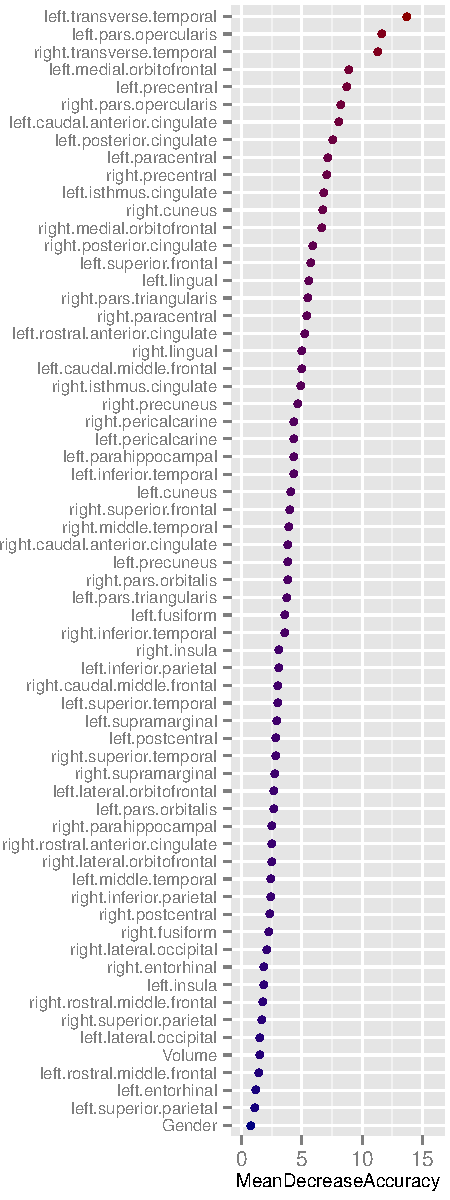
\includegraphics[width=40mm]{importanceANTs.pdf} &
  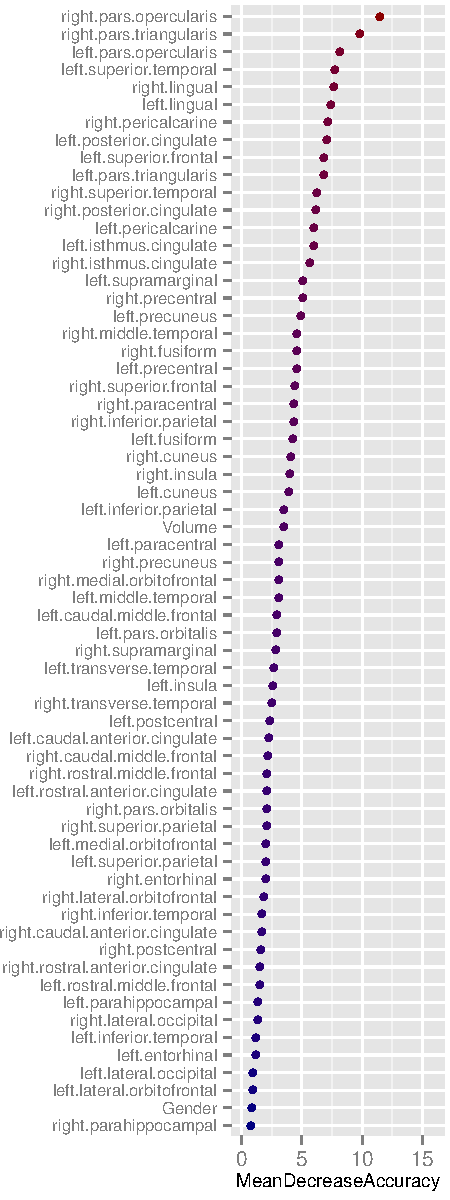
\includegraphics[width=40mm]{importanceFreeSurfer.pdf}
  \end{tabular}
  \caption{Regional importance random forest plots for (left) ANTs and (right) FreeSurfer using ``MeanDecreaseAccuracy'' ranking all model variables specified by Equation (\ref{eq:lmage}).
           }
  \label{fig:importance}
\end{figure}


{\color{blue}{To further elucidate the regional differences in predictive power
specifically in the random forest model, we provide variable importance
plots for both pipelines using the mean decrease in accuracy measure in 
Figure \ref{fig:importance}.  During random forest
model construction (specifically the out-of-bag error calculation stage), 
the decrease in prediction accuracy with the omission of a 
single feature or variable is tracked and averaged. Thus, those features which 
have the greatest decrease in mean accuracy are considered to be the most discriminative.
It should be noted that correlative effects are not considered in the rankings.
}}


\begin{figure*}
  \centering
  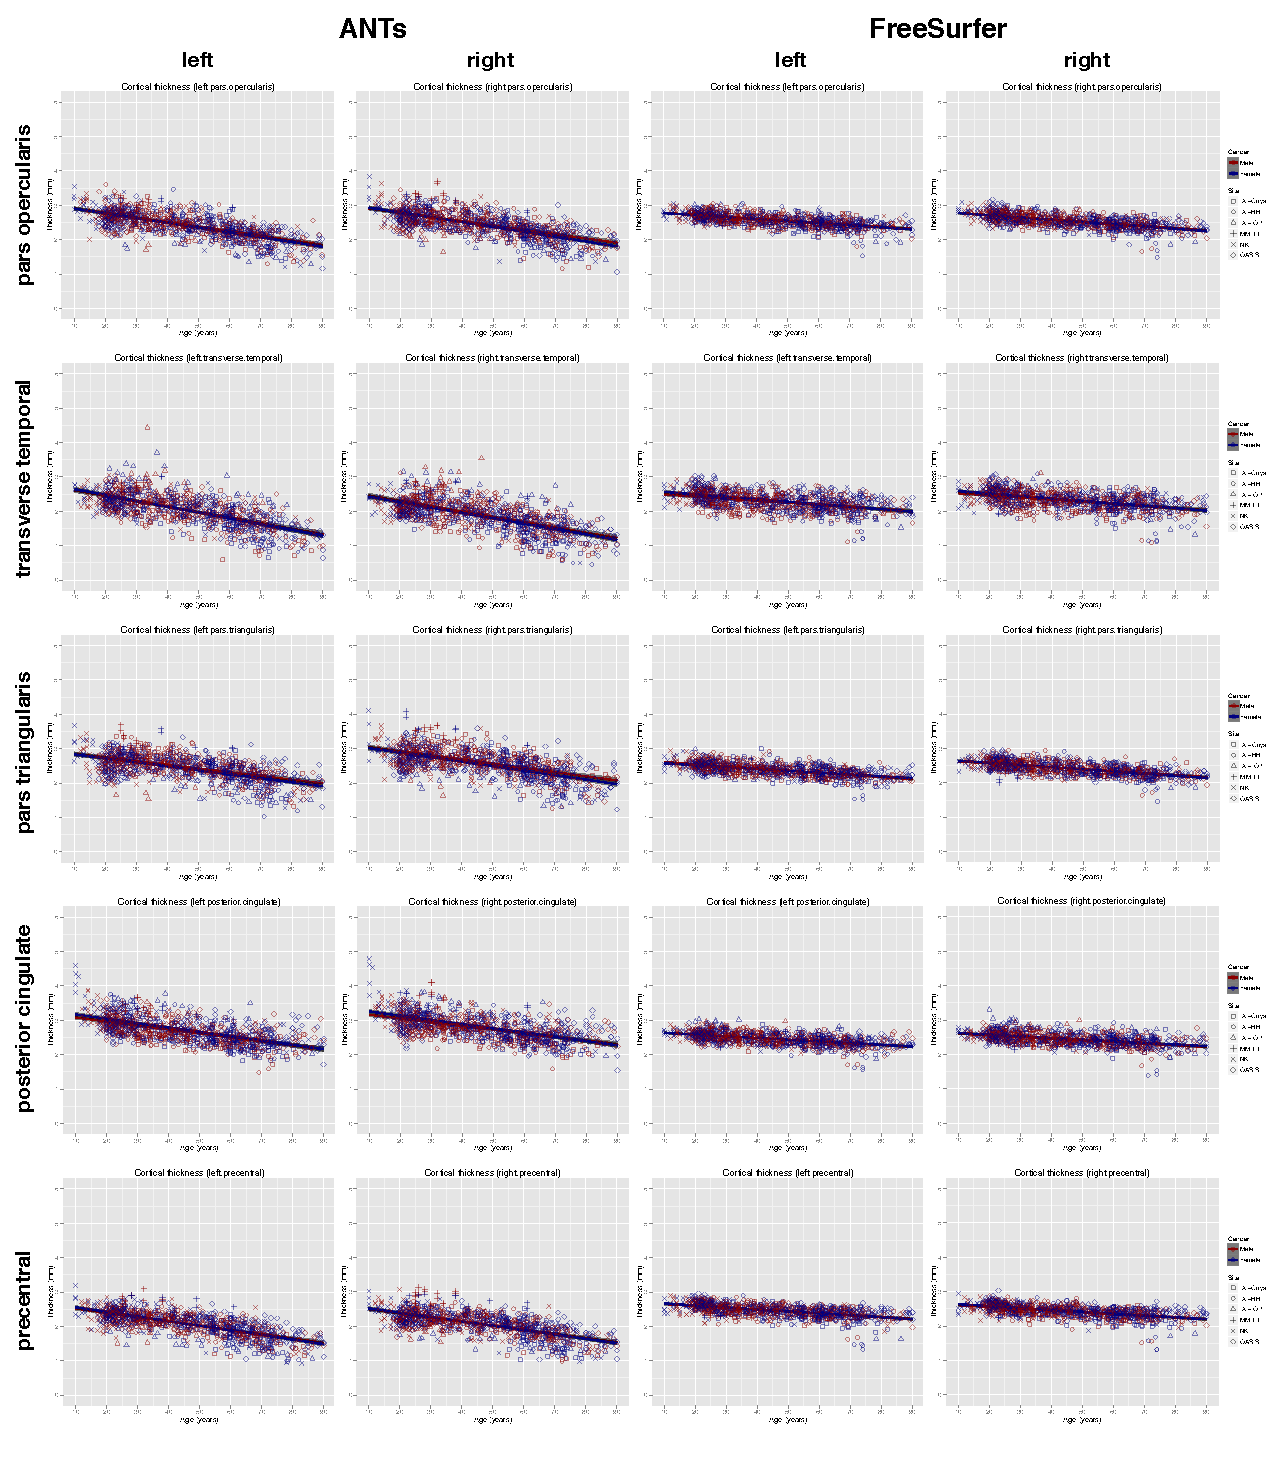
\includegraphics[width=180mm]{rfImportanceRegions.pdf}
  \caption{Age vs. thickness plots for regions that are most relevant for age prediction.  
           These are the most discriminative regions across both methods as determined 
           by random forest importance measurements (cf Figure 7). Note that all regional 
           plots for both ANTs and FreeSurfer are available online (see Appendix)
           along with corresponding surface-based rendering of thickness values.                
           }
  \label{fig:importanceRegions}
\end{figure*}


\subsection{Gender prediction assessment}

\begin{figure*}[htb]
  \centering
  \begin{tabular}{c}
  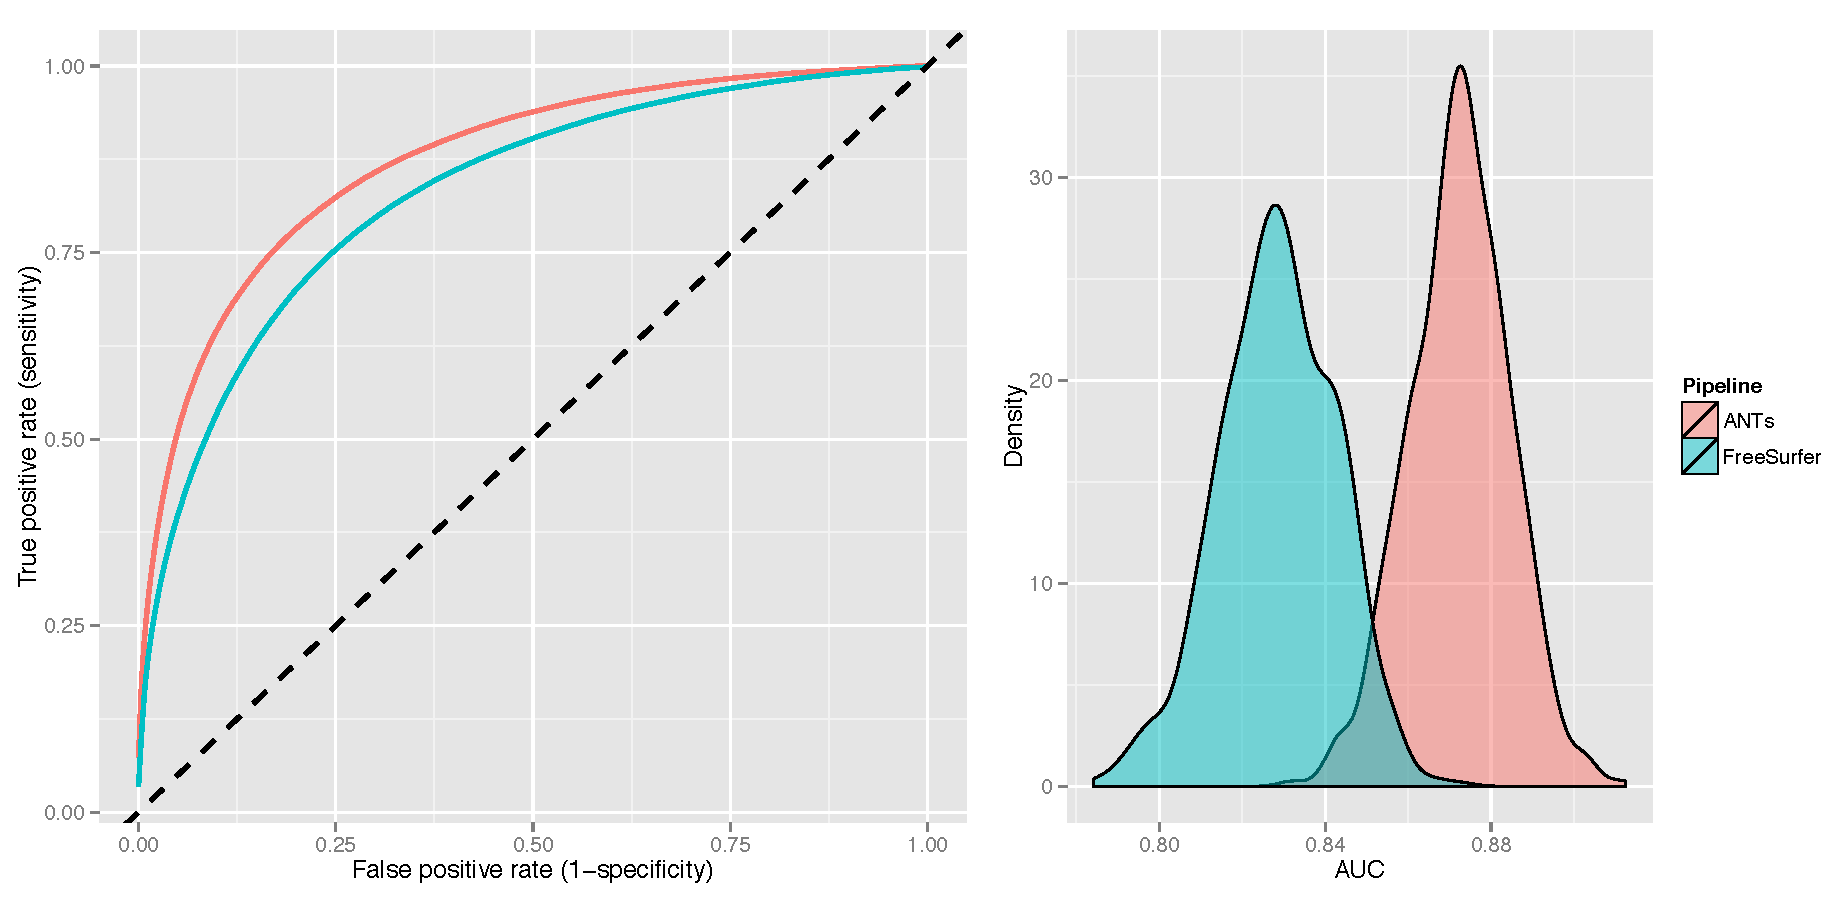
\includegraphics[width=140mm]{genderPrediction.pdf}
  \end{tabular}
  \caption{Average ROC curve and corresponding AUC distributions
  for gender prediction using ANTs and FreeSurfer thickness values.
  Values were averaged for 1000 permutations resulting in mean
  values of ANTs$_{AUC} =0.87$ and FreeSurfer$_{AUC} =0.83$
  ($p < 10^{-16}$).
  }
  \label{fig:genderPrediction}
\end{figure*}

We also performed a similar prediction assessment using gender
as the regressand.   The binomial generalized linear model is
\begin{align}
  GENDER \sim VOLUME + AGE + \sum_{i=1}^{62} T(DKT_{i})
\end{align}
where $T(DKT_{i})$ is the average thickness value in region $DKT_{i}$
{\color{blue}{and $VOLUME$ is total intracranial volume}}.
We then characterized performance using a ROC curve for both methods 
(see Figure \ref{fig:genderPrediction}) where we averaged over 1000
permutations.  The mean area under the curve (AUC) for
both methods was also quantified with values of ANTs$_{AUC} =0.87$ and 
FreeSurfer$_{AUC} =0.83$.

   

\subsection{Computation time}

%\begin{figure}[htb]
%  \centering
%  \begin{tabular}{c}
%  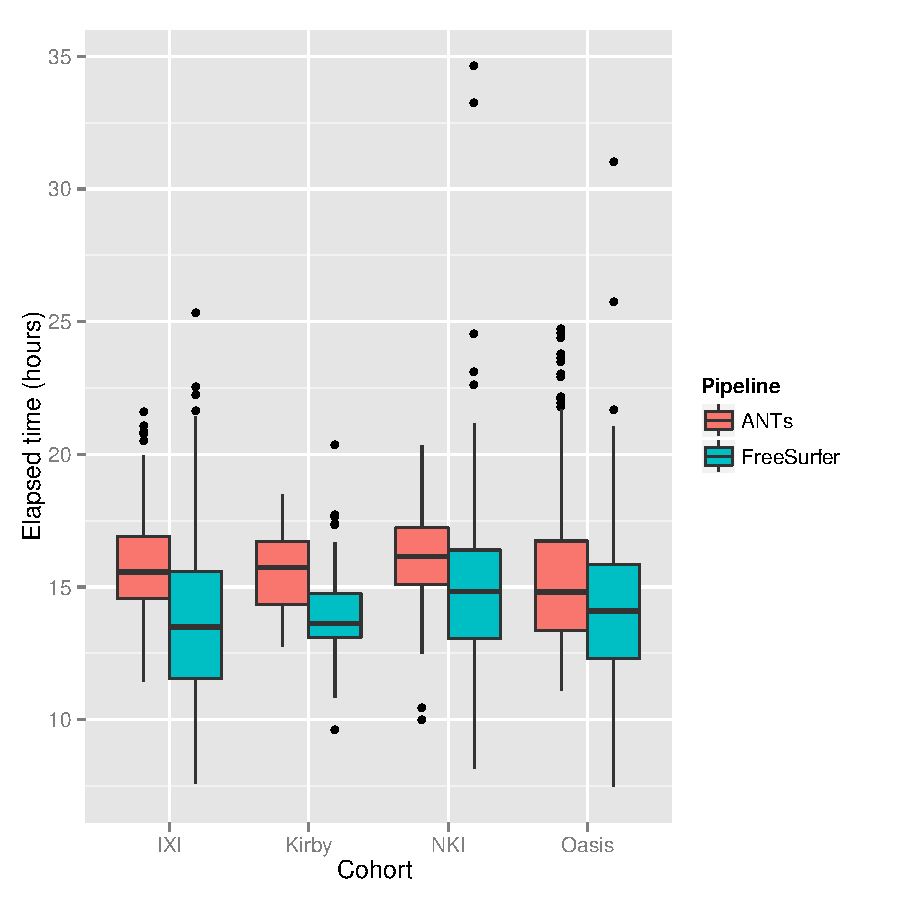
\includegraphics[width=90mm]{Times.pdf}
%  \end{tabular}
%  \caption{\baselineskip 12pt Elapsed time across data sets for ANTs and 
%           FreeSurfer processing.  Averaged over all cohorts, ANTs required $15.7 \pm 2.0$ hours per subject and FreeSurfer required $14.1 \pm 2.9$ hours per subject.
%           }
%  \label{fig:times}
%\end{figure}

All images underwent the ANTs and FreeSurfer pipeline processing 
using the computational cluster at the University of Virginia.  
Processing times varied approximately between 10--20 hours per subject
for both pipelines for the entire cortical thickness estimation procedure
although ANTs processing, on average, took slightly longer.  Averaged over all cohorts, ANTs required 
$15.7 \pm 2.0 $ hours per subject and FreeSurfer required $14.1 \pm 2.9$ hours per subject.

The propagation of the DKT labels to each subject using label fusion as described earlier
was performed in parallel and took anywhere between 40 and 80 hours per 
subject for 16 serial image registrations and application of the joint label fusion algorithm \citep{wang2013}. 
For each subject, 20 atlas registrations are used to generate the labeling 
for that subject.  Therefore to do the MALF labeling for the entire cohort, approximately 
$1200 \times 20 = 24000$ registrations were performed.  
The {\tt antsMalfLabeling.sh} script mentioned earlier parallelizes
the registration component which decreases the time for parallel computation platforms.
 
 
 

